\chapter{Bayesian Machine Learning}

\section{Bayes Theorem}

\subsubsection{Bayesian Inference Example}

In our lecture slides, we demonstrate how focusing solely on likelihoods can be misleading. Consider a bird described as \textbf{``white with an orange beak''}. This description seems to fit seagulls better than pigeons. However, when we factor in the prior probability of encountering a pigeon versus a seagull, the prior for pigeons may be significantly higher. According to Bayes' theorem, this prior can outweigh the likelihood, leading us to conclude that the bird is more likely a pigeon.

\ex{Pigeons and Seagulls}{\begin{itemize}
        \footnotesize
        \item \textbf{Population Data in London}:
              \begin{itemize}
                  \item Population of Pigeons: $3{,}000{,}000$ (97\%)
                  \item Population of Seagulls: $100{,}000$ (3\%)
              \end{itemize}
        \item \textbf{Likelihoods Based on Description}:
              \begin{itemize}
                  \item Probability that a pigeon is \textbf{white with an orange beak}: $P(\text{White with Orange Beak} \mid \text{Pigeon}) = 0.01$ (1\%)
                  \item Probability that a seagull is \textbf{white with an orange beak}: $P(\text{White with Orange Beak} \mid \text{Seagull}) = 0.90$ (90\%)
              \end{itemize}
        \item \textbf{Applying Bayes' Theorem}:
              \[
                  P(\text{Pigeon} \mid \text{White with Orange Beak}) = \frac{P(\text{White with Orange Beak} \mid \text{Pigeon}) \cdot P(\text{Pigeon})}{P(\text{White with Orange Beak})}
              \]
              where:
              \begin{align*}
                  P(\text{White with Orange Beak}) & = P(\text{White with Orange Beak} \mid \text{Pigeon}) \cdot P(\text{Pigeon})         \\
                                                   & \quad + P(\text{White with Orange Beak} \mid \text{Seagull}) \cdot P(\text{Seagull})
              \end{align*}  Plugging in the values:
              \[
                  P(\text{White with Orange Beak}) = (0.01)(0.97) + (0.90)(0.03) = 0.0097 + 0.027 = 0.0367
              \]
              Therefore:
              \[
                  P(\text{Pigeon} \mid \text{White with Orange Beak}) = \frac{0.01 \times 0.97}{0.0367} \approx 0.264
              \]
        \item \textbf{Interpretation of Results}:
              Despite the high likelihood that a \textbf{white with an orange beak} bird is a seagull, the overwhelming prior probability of encountering a pigeon in London results in a higher posterior probability of the bird being a pigeon. Specifically, there is approximately a 26.4\% chance the bird is a pigeon and a 73.6\% chance it is a seagull.
    \end{itemize}}

\begin{itemize}
    \item \textbf{Incorporation of Prior Beliefs:} New evidence updates our existing beliefs rather than determining them in isolation.
    \item \textbf{Expression of Uncertainty:} Bayesian predictions inherently account for uncertainty in the parameters.
\end{itemize}

Bayesian learning allows us to express uncertainties about predictions and other quantities by updating our beliefs based on observed data.

\hl{The critical observation of Bayes in situations like these is that data should not determine our belief in a vacuum. We should always consider data as updating our current beliefs}

\defb{Prior}{The prior distribution, \( P(\theta) \), represents our beliefs about the parameter \( \theta \) before observing any data.}

\defb{Likelihood}{The likelihood, \( P(\mathcal{D}|\theta) \), represents the probability of observing the data \( \mathcal{D} \) given the parameter \( \theta \).}

Recall Bayes' theorem:

\[
    P(\theta|\mathcal{D}) = \frac{P(\mathcal{D}|\theta)P(\theta)}{P(\mathcal{D})}
\]

Where:
\begin{itemize}
    \item \( P(\theta|\mathcal{D}) \) is the posterior distribution.
    \item \( P(\mathcal{D}|\theta) \) is the likelihood.
    \item \( P(\theta) \) is the prior.
    \item \( P(\mathcal{D}) \) is the evidence.
\end{itemize}

The posterior distribution \( P(\theta|\mathcal{D}) \) quantifies the probability of the parameter \( \theta \) after observing the dataset \( \mathcal{D} \).

\subsection{Motivating Bayes Theorem}

Consider the classical scenario of estimating the probability of heads in a biased coin. We model the result of a coin flip as a Bernoulli random variable:

\[
    p(X=x) =
    \begin{cases}
        \theta     & \text{if } x = 1 \text{ (heads)} \\
        1 - \theta & \text{if } x = 0 \text{ (tails)}
    \end{cases}
\]

In previous notes, the Maximum Likelihood Estimate (MLE) for \( \theta \) is:

\[
    \theta^{\mathrm{MLE}} = \frac{1}{n} \sum_{i=1}^{n} x_i
\]

Assume the observed data is \( \mathcal{D} = \{1, 1, 1, 1\} \). Then, it is clear (without having to take the MLE) that

\begin{equation}
    \theta^{\mathrm{MLE}} = 1 \label{eq:mle_coin_overfit}
\end{equation}

This suggests complete certainty in the coin always landing heads, \textbf{which is unrealistic}.\footnote{For many, having overzealous faith in the coin always landing heads with 0 probability of tails seems like an absurd conclusion, the result of an overly simplistic mathematical model. This is due to our prior knowledge that designing a two-sided coin with probability 1 of landing on heads would be physically very challenging. In fact, there is some debate as to weather or not a biased coin could be manufactured in the first place, see \href{https://www.stat.berkeley.edu/ nolan/Papers/dice.pdf}{here}.} Bayesian inference addresses this by incorporating prior knowledge. Before observing any data, a rational assumption might be \( \theta = 0.5 \). In the Bayesian framework, this is represented by the prior \( P(\theta) \).

\subsection{Selecting the Prior Distribution}

Selecting an appropriate prior distribution is crucial and debated among statisticians. There are two main perspectives:

\begin{itemize}
    \item \textbf{Subjective Bayesian:} Encodes prior knowledge based on experience or previous data.
    \item \textbf{Objective Bayesian:} Chooses priors that minimally influence the inference, primarily capturing uncertainty.
\end{itemize}

For this module, we adopt a subjective Bayesian approach, selecting priors that reflect our knowledge. A common simplifying assumption in Bayesian modeling is to omit the denominator \( P(\mathcal{D}) \), also known as the evidence, for analytical convenience:

\[
    P(\theta|\mathcal{D}) \propto P(\mathcal{D}|\theta)P(\theta)
\]

\defb{Distribution being a Conjugate Prior}{
    A distribution is a conjugate prior for a likelihood if the product of the prior and likelihood yields a distribution from the same family as the prior.\bigskip

    Sometimes it is also used to simply describe a prior whose product with the likelihood gives us a closed-form posterior distribution.
}

When choosing a prior, it is beneficial to select a distribution that allows the posterior to remain in the same family. Recall for a Bernoulli distribution, the parameter $\theta$ which is the likelihood of observation $x$, is:

\[
    p(x|\theta) = \theta^x(1-\theta)^{1-x}
\]

Assume that the data is i.i.d, then the probability of our dataset with be a product of powers of $\theta$ and $1-\theta$, which grow as we observe more data. In our coin flip example for  \( \mathcal{D} = \{1, 1, 1, 1\} \), the likelihood is:

\[
    P(\mathcal{D}|\theta) = \theta^4(1 - \theta)^0 = \theta^4
\]

Where maximising the likelihood is $\theta = 1$. Given this is our likelihood, it is intuitive that we would want to express our prior as a product of powers of $\theta$ and $1-\theta$ as well. This is where the Beta distribution comes in. For a Bernoulli likelihood, the Beta distribution serves as a conjugate prior:

\[
    P_{\mathrm{Beta}}(\theta) = \text{const.} \cdot \theta^{\alpha - 1}(1 - \theta)^{\beta - 1}
\]

% A sensible choice might be \( \alpha = 2 \) and \( \beta = 2 \), centering the prior around \( \theta = 0.5 \) and avoiding extreme probabilities of \( \theta = 0 \) or \( \theta = 1 \).

\subsection{Conjugate Prior for Bernoulli Likelihood}\label{sec:conjugate_ridge}

A distribution is a conjugate prior for a likelihood if the posterior distribution belongs to the same family as the prior. For the Bernoulli likelihood:

\[
    P(X=x|\theta) = \theta^x (1 - \theta)^{1 - x}
\]

Given the data \( \mathcal{D} = \{1, 1, 1, 1\} \), the likelihood becomes:

\[
    P(\mathcal{D}|\theta) = \theta^4 (1 - \theta)^0 = \theta^4
\]

\begin{marginfigure}
    \centering
    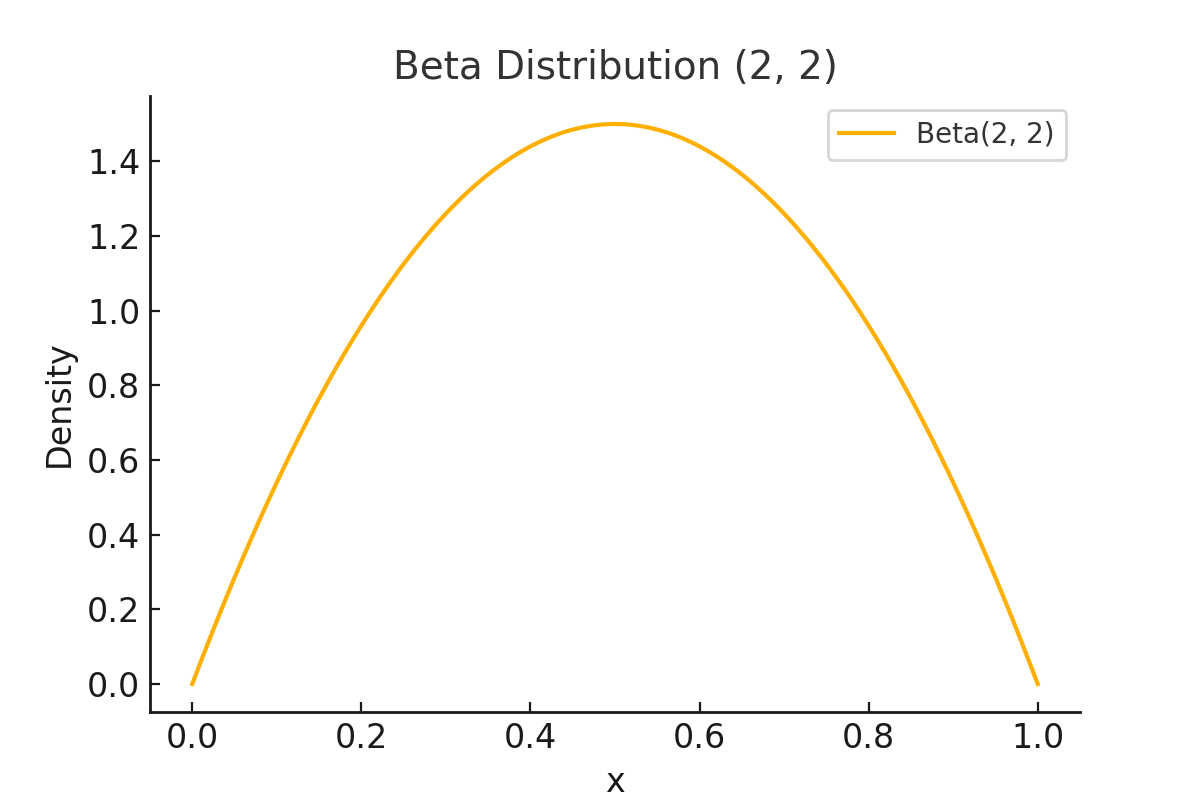
\includegraphics[width=\linewidth]{img/11_Beta_2_2.png}
    \caption{Posterior Distribution for Beta(2, 2)}
    \label{fig:beta_prior}
\end{marginfigure}


It is sensible to assume that the coin would be fair to start with. We choose a Beta prior with \( \alpha = 2 \) and \( \beta = 2 \), as it has a mode/mean at 0.5 and puts the prior density away from the unlikely case of \( \theta = 0 \) or \( \theta = 1 \) :

\[
    P(\theta) = \theta^{1} (1 - \theta)^{1}
\]

To arrive at our posterior distribution: recall that the posterior distribution is proportional to the product of the likelihood and prior:
\[
    p(\theta \mid D) \propto p(D \mid \theta)p(\theta)
\]


Using the Beta prior density with parameters \(\alpha = 2\) and \(\beta = 2\), we write:
\[
    p(\theta \mid D) \propto p(D \mid \theta) \theta^{\alpha-1} (1 - \theta)^{\beta-1} = p(D \mid \theta) \theta^1 (1 - \theta^1)
\]


Now we expand the likelihood and incorporate the dataset \(D\): \marginnote{
    \raggedright

    The \textbf{Beta distribution} is a continuous distribution over $[0, 1]$, parameterised by shape parameters $\alpha$ and $\beta$. Its PDF is:
    \[
        f(x \mid \alpha, \beta) = \frac{\Gamma(\alpha + \beta)}{\Gamma(\alpha) \Gamma(\beta)} x^{\alpha - 1} (1 - x)^{\beta - 1}
    \]
    where $0 < x < 1$. \bigskip

    The mean of the Beta distribution is:
    \[
        \mathbb{E}[X] = \frac{\alpha}{\alpha + \beta}
    \]
}





\begin{align*}
    p(\theta|\mathcal{D}) & \propto p(\mathcal{D}|\theta)\theta^{1}(1-\theta)^{1}                                                                                   \\
                          & = \left(\prod_{x^{(i)}\in\mathcal{D}}(\theta)^{x^{(i)}}(1-\theta)^{x^{(i)}}\right)\theta^{1}(1-\theta)^{1}                              \\
                          & = \left((\theta)^{\sum_{x^{(i)}\in\mathcal{D}}x^{(i)}}(1-\theta)^{n-\sum_{x^{(i)}\in\mathcal{D}}x^{(i)}}\right)\theta^{1}(1-\theta)^{1} \\
                          & = (\theta)^{1+\sum_{x^{(i)}\in\mathcal{D}}x^{(i)}}(1-\theta)^{1+n-\sum_{x^{(i)}\in\mathcal{D}}x^{(i)}}                                  \\
                          & = (\theta)^{1+4}(1-\theta)^{1+0}
\end{align*}



\bigskip
Thus, the posterior is a Beta distribution with parameters \( \alpha' = 6 \) and \( \beta' = 2 \).

\[
    P(\theta|\mathcal{D}) \propto \theta^{5}(1-\theta)^{1}
\]

So, at the end, we have that our posterior is simply a beta distribution with parameter 5 and 1. Notice in Figure \ref{fig:beta_posterior} that now our posterior mean is $\frac{6}{6+2} = 0.75$ rather than 1($\theta$ calculated by maximum likelihood on sample data)\footnote{We calculated the MLE for seeing $\{1,1,1,1\}$ coin flips in \ref{eq:mle_coin_overfit}. \hl{MLE leads to severe overfitting especially when we have little data!}}. In our case, when setting a prior that tries to `keep things sensible' by assuming coins are fair, the biasedness of the coin is reduced. \bigskip


Moreover, we have some clear uncertainty about this. For example, we can see that we assign roughly 10\% chance that the true probability is less than 0.6. It is unclear at first glance how to reason about these uncertainties in the frequentist case. \bigskip

We still need to compute the normalising constant – however for the Beta distribution, this is a known value, so we can compute the posterior directly:

\[
    P(\theta|\mathcal{D}) = \frac{\Gamma(6+2)}{\Gamma(6)\Gamma(2)} \theta^{6-1} (1-\theta)^{2-1}
\]

Our normalising constant is $\frac{\Gamma(6+2)}{\Gamma(6)\Gamma(2)} = \frac{7!}{5!1!} = 7*6 = 42$.


\begin{marginfigure}
    \centering
    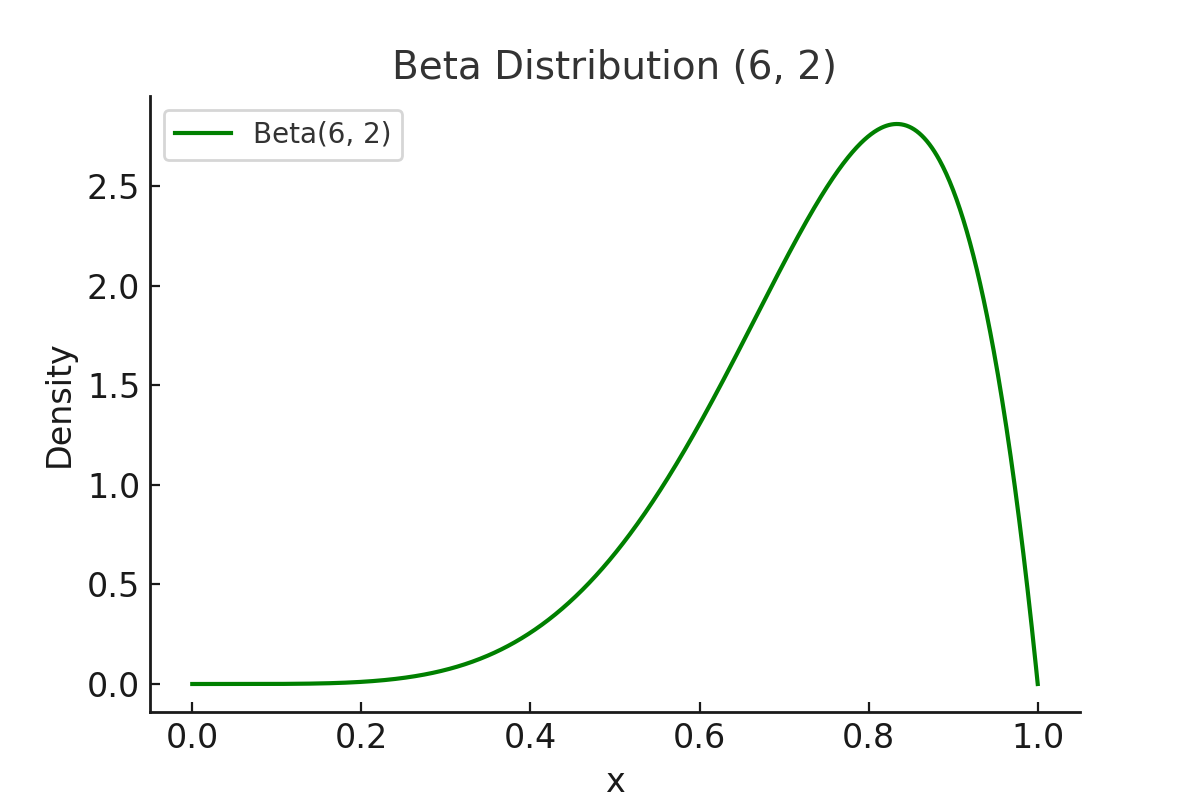
\includegraphics[width=\linewidth]{img/11_Beta_6_2.png}
    \caption{Posterior Distribution for Beta(6, 2)}
    \label{fig:beta_posterior}
\end{marginfigure}


\subsection{Equating Coefficients for Inference in Conjugate Models}

The technique of equating coefficients is powerful in conjugate models. The steps are:

\begin{itemize}
    \item \textbf{Select Conjugate Prior and Likelihood:} Choose a prior and likelihood that belong to conjugate families.
    \item \textbf{Expand and Simplify:} Multiply the prior and likelihood, then simplify the expression.
    \item \textbf{Match Posterior Form:} Compare the resulting expression to the known form of the posterior and solve for its parameters.
\end{itemize}

In our example, knowing that the Beta distribution is conjugate to the Bernoulli likelihood allowed us to directly identify the posterior parameters by matching the exponents of \( \theta \) and \( (1 - \theta) \).

\subsection{Posterior Predictive Distribution}
\marginnote{\sn{}{In machine learning, we are not just interested in computing a posterior distribution– we are interested in using the posterior distribution to make predictions about unseen objects and events.}}

Beyond computing the posterior, Bayesian inference allows us to make predictions about unseen data. Assume an unsupervised learning scenario, with some unseen feature vector $\bm{x}$. The probability we are interested in is, $p(x^*|\mathcal{D})$, or in words, the probability distribution of feature $\bm{x}$ given the data $\mathcal{D}$. \bigskip

We have access to the posterior distribution of the parameters, $p(\theta|\mathcal{D})$. We can use this to compute the posterior predictive distribution, $p(x^*|\mathcal{D})$:

\[
    p(x^{*}|{\mathcal D},\theta)=\int_{\theta}p(x^{*}|\theta)p(\theta|{\mathcal D})d\theta
\]

This is usually done for generative models, since we do not have prediction labels $y$.\bigskip
% This equation helps us make predictions, and also allows us to evaluate our model given a held out set of data. For example, we may want to compute the log likelihood of seeing new data given our model. \bigskip

In supervised learning, we are interested in predicting the label $y$ given a feature vector $x$. The posterior predictive distribution is:

\[
    P(y|x^*, \mathcal{D}) = \int_{\theta} P(y|x^*, \theta) P(\theta|\mathcal{D}) \, d\theta
\]

This integral accounts for uncertainty in \( \theta \) by averaging over the posterior distribution. In practice, for conjugate models, this integral often has a closed-form solution.

\section{Bayesian Linear Regression}



\sn{Extract from Deisenroth et al (2020):}{
    Bayesian linear regression pushes the idea of the parameter prior a step further and does not even attempt to compute a point estimate of the parameters, but instead the full posterior distribution over the parameters is taken into account when making predictions. This means we do not fit any parameters, but we compute a mean over all plausible parameters settings (according to the posterior).

}
In Bayesian machine learning models, we have two critical components:
\defb{Likelihood}{The likelihood \( P(\boldsymbol{y}|\boldsymbol{x}, \theta) \) models the observational noise of the process. Observed outputs $y$ are not perfectly determined by inputs $x$, but are instead corrupted by noise. \bigskip


    The likelihood assumes that given $\bm{X}$ and parameters $\theta$, the output $y$ follows the normal distribution:
    \[
        P( \boldsymbol{y}|\boldsymbol{x}, \theta ) = \mathcal{N}(\boldsymbol{X}^\top \theta, \sigma^2)
    \]



}
\defb{Prior}{The prior \( P(\theta) \) encodes our beliefs about the parameters \( \theta \) before observing any data.}\marginnote{
    This is the case in Table \ref{tab:conjugate_priors} where our prior is Gaussian, our likelihood is Gaussian \textbf{with known variance}, and our posterior is Gaussian.}
\pagebreak

% As we have seen in previous exercises, the conjugate prior for the mean of a Gaussian with known variance is a Gaussian, so we know that in this case it will be analytically convenient to select a Gaussian prior:}

Consider the model:
\[
    \begin{array}{ll}
        \text{prior}      & P(\theta) = \mathcal{N}(0, \tau^2 \bm{I}),                                   \\[0.5em]
        \text{likelihood} & P(\bm{y} \mid \bm{X}, \theta) = \mathcal{N}(\bm{X} \theta, \sigma^2 \bm{I}).
    \end{array}
\]
\begin{marginfigure}
    \centering
    \begin{tikzpicture}[
            node distance=0.5cm and 0.5cm,
            every node/.style={draw, circle, minimum size=0.7cm, font=\sffamily},
            every edge/.style={-Stealth, thick, line width=1.5pt}
        ]

        % Nodes
        \node (theta) {$\theta$};
        \node[above left=of theta, draw=none] (mu) {$\mu = 0$};
        \node[above right=of theta, draw=none] (tau2) {$\tau^2 \bm{I}$};
        \node[below=of theta] (y) {$y$};
        \node[left=of y, draw=none] (X) {$\bm{X}$};
        \node[right=of y, draw=none] (sigma) {$\sigma$};

        % Edges
        \draw[->] (mu) -- (theta);
        \draw[->] (tau2) -- (theta);
        \draw[->] (theta) -- (y);
        \draw[->] (X) -- (y);
        \draw[->] (sigma) -- (y);

    \end{tikzpicture}
    \caption{Graphical model for Bayesian linear regression.}
    \label{fig:bayesian_linear_regression}
\end{marginfigure}


\begin{itemize}
    \item \textbf{Likelihood:}
          \begin{itemize}
              \item Assumes Gaussian noise in supervised learning.
              \item For a single-dimensional response \( y \), the likelihood is:
                    \[
                        P(\boldsymbol{y}|\boldsymbol{X}, \theta) = \mathcal{N}(\boldsymbol{X}\theta, \sigma^2 \mathbf{I})
                    \]
              \item In matrix form:
                    \[
                        P(\boldsymbol{y}|\boldsymbol{X}, \theta) = \frac{1}{(2\pi\sigma^2)^{N/2}} \exp\left( -\frac{1}{2\sigma^2} (\boldsymbol{y} - \boldsymbol{X}\theta)^\top (\boldsymbol{y} - \boldsymbol{X}\theta) \right)
                    \]
          \end{itemize}

    \item \textbf{Prior:}
          \begin{itemize}
              \item Our parameter vector $ \theta $ is now a random variable.
              \item Defined as:
                    \[
                        P(\theta) = \mathcal{N}(0, \tau^2 \mathbf{I})
                    \]\marginnote{$\bm{I}$ is the $k \times k$ identity matrix, where our prior is an isotropic Gaussian with variance $\tau^2$.}



              \item In expanded form:
                    \[
                        P(\theta) = \frac{1}{(2\pi\tau^2)^{k/2}} \exp\left( -\frac{1}{2\tau^2} \theta^\top \theta \right)
                    \]
          \end{itemize}
\end{itemize}

\marginnote{
    \defsb{Isotropic Gaussian}{
        An isotropic Gaussian is one where the covariance matrix \(\Sigma\) can be represented as:
        \[
            \Sigma = \sigma^2 I
        \]
        \begin{itemize}
            \item \(I\): The Identity matrix.
            \item \(\sigma^2\): The scalar variance.
        \end{itemize}
        \smallskip
        \textbf{Q: Why do we want to represent the covariance matrix in this form?} \bigskip

        \textbf{A:} As the dimensions of a multivariate Gaussian grow:
        \begin{itemize}
            \item The mean \(\mu\) follows a linear growth.
            \item The covariance matrix \(\Sigma\) grows quadratically in terms of the number of parameters.
        \end{itemize}
        This quadratic growth is computationally expensive. Representing the covariance as a diagonal matrix simplifies computations significantly.
    }}

We will now explore two ways of deriving the Bayesian posterior for our model.
\subsection{Deriving the Posterior via Densities (Easy)}

To compute the posterior distribution \( P(\theta|\mathcal{D}) \), we apply Bayes' theorem:

\[
    P(\theta|\mathcal{D}) \propto P(\mathcal{D}|\theta) P(\theta)
\]

Substituting the likelihood and prior:

\[
    P(\theta|\mathcal{D}) \propto \exp\left( -\frac{1}{2\sigma^2} (\boldsymbol{y} - \boldsymbol{X}\theta)^\top (\boldsymbol{y} - \boldsymbol{X}\theta) \right) \exp\left( -\frac{1}{2\tau^2} \theta^\top \theta \right)
\]

Expanding the quadratic terms:

\begin{align*}
    \log P(\theta|\mathcal{D}) & \propto -\frac{1}{2\sigma^2} \left( \theta^\top \boldsymbol{X}^\top \boldsymbol{X} \theta - 2 \boldsymbol{y}^\top \boldsymbol{X} \theta + \boldsymbol{y}^\top \boldsymbol{y} \right) - \frac{1}{2\tau^2} \theta^\top \theta                \\
                               & = -\frac{1}{2} \theta^\top \left( \frac{1}{\sigma^2} \boldsymbol{X}^\top \boldsymbol{X} + \frac{1}{\tau^2} \mathbf{I} \right) \theta + \frac{1}{\sigma^2} \boldsymbol{y}^\top \boldsymbol{X} \theta + \frac{1}{2\sigma^2}\bm{y}^\top\bm{y}
    \\
                               & \propto \theta^\top \left(  \tau^2 \boldsymbol{X}^\top \boldsymbol{X} +\sigma^2\mathbf{I} \right) \theta - \tau^2 \boldsymbol{y}^\top \boldsymbol{X} \theta +
    \text{const.}
\end{align*}

Recognising the quadratic form, the posterior is Gaussian with: \marginnote{
    \raggedright
    We can write any Gaussian distribution as:
    $$\begin{aligned}\log\left(\mathcal{N}(\theta;\boldsymbol{\mu},\boldsymbol{\Sigma})\right)&\propto(\theta-\boldsymbol{\mu})\boldsymbol{\Sigma}^{-1}(\theta-\boldsymbol{\mu})\end{aligned}$$

    $$\begin{aligned}&=\theta^{\top}\boldsymbol{\Sigma}^{-1}\theta-2\theta^{\top}\boldsymbol{\Sigma}^{-1}\boldsymbol{\mu}+\boldsymbol{\mu}^{\top}\boldsymbol{\Sigma}^{-1}\boldsymbol{\mu}\\&=\theta^{\top}\boldsymbol{\Sigma}^{-1}\theta-2\theta^{\top}\boldsymbol{\Sigma}^{-1}\boldsymbol{\mu}+\mathrm{const.}\end{aligned}$$

}

\[
    \boldsymbol{\Sigma}^{-1}=(\tau^2\boldsymbol{X}^\top\boldsymbol{X}+\sigma^2\mathbf{I})
\]

\[
    2\theta^\top\boldsymbol{\Sigma}^{-1}\boldsymbol{\mu}=2\tau^2\boldsymbol{y}^\top\boldsymbol{X}\theta \quad\Rightarrow\quad\boldsymbol{\mu}=\tau^2\boldsymbol{\Sigma}\boldsymbol{X}^\top\boldsymbol{y}
\]

Thus, the posterior distribution is:

\[
    P(\theta|\mathcal{D}) = \mathcal{N}\big(\theta;\tau^2\boldsymbol{\Sigma}\boldsymbol{X}^\top\boldsymbol{y},(\tau^2\boldsymbol{X}^\top\boldsymbol{X}+\sigma^2\mathbf{I})^{-1}\big)
\]

\pagebreak\subsubsection{Interpreting Posterior Values}

\begin{itemize}
    \item \textbf{Covariance Matrix \( \boldsymbol{\Sigma} \):}
          \begin{itemize}
              \item $$\mathbf{\Sigma}=\left(\frac{1}{\sigma^{2}}\mathbf{X}^{\top}\mathbf{X}+\sigma^{2}\mathbf{I}\right)^{-1}$$\marginnote{Posterior, so $\sigma$ not $\tau$}
              \item Must be invertible for the posterior to be well-defined.
              \item \( \tau^2\boldsymbol{X}^\top \boldsymbol{X} \) is positive semi-definite. \( \sigma^2 \mathbf{I} \) is positive definite if \( \sigma^2 > 0 \).
              \item Then, a positive definite matrix plus a positive semi-definite matrix is positive definite, thus invertible.
          \end{itemize}

    \item \textbf{Mean \( \boldsymbol{\mu} \):}
          \begin{itemize}
              %   \item $$\boldsymbol{\mu}=\tau^{2}\boldsymbol{\Sigma}\boldsymbol{X}^{\top}\boldsymbol{y}$$
              \item \begin{align*}
                        \bm{\mu} & = \tau^2 \Sigma \bm{X}^\top \bm{y}                                                            \\
                                 & = \tau^2 \big( \tau^2 \bm{X}^\top \bm{X} + \sigma^2 \bm{I} \big)^{-1} \bm{X}^\top \bm{y}      \\
                                 & = \left( \bm{X}^\top \bm{X} + \frac{\sigma^2}{\tau^2} \bm{I} \right)^{-1} \bm{X}^\top \bm{y}.
                    \end{align*}

              \item This corresponds to the Maximum A Posteriori (MAP) estimate for bayesian linear regression, \textbf{and this is equal to the ridge regression solution.} \marginnote{This is why the bayesian linear regression solution didn't overfit in the previous example \ref{sec:conjugate_ridge}.}
              \[
              \theta^{\text{MAP}} = \left( \bm{X}^\top \bm{X} + \frac{\sigma^2}{\tau^2} \bm{I} \right)^{-1} \bm{X}^\top \bm{y}
                \]

          \end{itemize}
\end{itemize}

\subsection{Deriving the Posterior via Joint Gaussian}

An alternative method involves modeling the joint distribution of \( \theta \) and \( \boldsymbol{y} \) as Gaussian.

\thm{Marginalisation}{
    Given a Gaussian random variable:
    \[
        \mathcal{N}\left(
        \begin{bmatrix}
                a \\ b
            \end{bmatrix},
        \begin{bmatrix}
                \mu_a \\ \mu_b
            \end{bmatrix},
        \begin{bmatrix}
                \Sigma_{a,a} & \Sigma_{a,b} \\
                \Sigma_{b,a} & \Sigma_{b,b}
            \end{bmatrix}
        \right)
    \]
    The marginal distribution of \(a\) is given by:
    \[
        P(a) = \mathcal{N}(a; \mu_a, \Sigma_{a,a}).
    \]
}

\thm{Conditioning}{
    Given a Gaussian random variable:
    \[
        \mathcal{N}\left(
        \begin{bmatrix}
                a \\ b
            \end{bmatrix},
        \begin{bmatrix}
                \mu_a \\ \mu_b
            \end{bmatrix},
        \begin{bmatrix}
                \Sigma_{a,a} & \Sigma_{a,b} \\
                \Sigma_{b,a} & \Sigma_{b,b}
            \end{bmatrix}
        \right)
    \]
    The conditional distribution \(p(a|b)\) is given by:
    \[
        P(a|b) = \mathcal{N}(a; \mu_{a|b}, \Sigma_{a|b}),
    \]
    where:
    \[
        \mu_{a|b} = \mu_a + \Sigma_{a,b}\Sigma_{b,b}^{-1}(b - \mu_b),
        \quad
        \Sigma_{a|b} = \Sigma_{a,a} - \Sigma_{a,b}\Sigma_{b,b}^{-1}\Sigma_{b,a}.
    \]
}


\begin{itemize}
    \item \textbf{Define the Joint Distribution:} \marginnote{
              We change notation here such that $\Sigma_{a,b} = \mathbb{C}[a,b]$ and $\Sigma_{a,a} = \mathbb{V}[a]$.
          }
          \[
              P(\theta, \boldsymbol{y}) = \mathcal{N}\left(
              \begin{bmatrix} \theta \\ \boldsymbol{y} \end{bmatrix};
              \begin{bmatrix} \mathbb{E}_{p(\theta)}[\theta] \\ \mathbb{E}_{\boldsymbol{y}}[\boldsymbol{y}] \end{bmatrix},
              \begin{bmatrix} \mathbb{V}[\theta] & \mathbb{C}[\theta, \boldsymbol{y}] \\ \mathbb{C}[\boldsymbol{y}, \theta] & \mathbb{V}[\boldsymbol{y}] \end{bmatrix}
              \right)
          \]

    \item \textbf{Apply the Conditioning Theorem:}
          Using the theorem, the posterior \( p(\theta|\boldsymbol{y}) \) is:
          \[
              P(\theta|\boldsymbol{y}) = \mathcal{N}\left( \mu_{\theta|\boldsymbol{y}}, \Sigma_{\theta|\boldsymbol{y}} \right)
          \]
          where
          \begin{align*}
              \mu_{\theta|\boldsymbol{y}}    & = \mathbb{E}_{p(\theta)}[\theta] + \mathbb{C}[\theta, \boldsymbol{y}] \mathbb{V}[\boldsymbol{y}]^{-1} (\boldsymbol{y} - \mathbb{E}_{\boldsymbol{y}}[\boldsymbol{y}]), \\
              \Sigma_{\theta|\boldsymbol{y}} & = \mathbb{V}[\theta] - \mathbb{C}[\theta, \boldsymbol{y}] \mathbb{V}[\boldsymbol{y}]^{-1} \mathbb{C}[\boldsymbol{y}, \theta].
          \end{align*}

          We have:
          \begin{align*}
            \mathbb{E}[\bm{\theta}] &= \bm{0}, \quad \mathbb{V}[\bm{\theta}] = \bm{I}_n, \quad \mathbb{E}[\bm{y}] = \bm{0} \\
            \mathbb{V}[\bm{y}] &= \mathbb{V}[\bm{X\theta}] + \mathbb{V}[\bm{\epsilon}] \quad \text{(By independence)} \\
            \mathbb{V}[\bm{y}] &= \bm{X}^\top \bm{X} + \sigma^2 \quad \text{(By linearity of expectation)}
            \end{align*}

            \marginnote{Since \(\bm{\theta}\) is normally distributed, its expectation is linked to its covariance. Here, \(\mathbb{V}[\bm{\theta}]\) is the identity matrix \(\bm{I}_n\), which simplifies the computation of the covariance.
            }
          \begin{align*}
            \mathbb{C}(\bm{\theta}, \bm{y}) 
            &= \mathbb{E}[\bm{\theta} \bm{y}^\top] - \mathbb{E}[\bm{\theta}] \mathbb{E}[\bm{y}] \\
            &= \mathbb{E}[\bm{\theta} (\bm{X\theta} + \bm{\epsilon})^\top] \\
            &= \mathbb{E}[\bm{\theta} \bm{\theta}^\top \bm{X}^\top] + \mathbb{E}[\bm{\theta}] \mathbb{E}[\bm{\epsilon}] \\
            &= \bm{X}^\top
            \end{align*}

            


    \item \textbf{Substitute the Specific Covariances:}
            We substitute and are left with:
\[
p(\bm{\theta} \mid \bm{X}, \bm{y}) = \mathcal{N}\left(\bm{\theta}; \bm{X}^\top \left(\bm{X} \bm{X}^\top + \sigma^2 \bm{I} \right)^{-1} \bm{y}, \bm{I} - \bm{X}^\top \left(\bm{X} \bm{X}^\top - \sigma^2 \bm{I}\right) \bm{X} \right)
\]

            This is equivalent to:
\[
p(\bm{\theta} \mid \bm{X}, \bm{y}) = \mathcal{N}\left(\bm{\theta}; \left(\bm{X}^\top \bm{X} + \frac{1}{\sigma^2} \bm{I} \right)^{-1} \bm{X}^\top \bm{y}, \left(\frac{1}{\sigma^2} \bm{X}^\top \bm{X} + \bm{I} \right)^{-1} \right)
\]

         
  
\end{itemize}

% \egb{Posterior Equivalence}{
% Show that the posterior distribution derived via the Conditioning Theorem:

% {\footnotesize
% \[
%     \mathcal{N}\left(
%     \theta; \Phi(X)^\top \left[ \Phi(X) \Phi(X)^\top + \sigma^2 \mathrm{I}_N \right]^{-1} \boldsymbol{y},\
%     \left( \Phi(X)^\top \Phi(X) + \frac{\sigma^2}{\tau^2} \mathrm{I}_M \right)^{-1}
%     \right)
% \]
% }

% is identical to the posterior obtained via equating coefficients:
% \[
%     \mathcal{N}\left( \theta; \boldsymbol{\mu}, \boldsymbol{\Sigma} \right)
% \]
% where
% \[
%     \boldsymbol{\mu} = \boldsymbol{\Sigma} \left( \frac{1}{\sigma^2} \Phi(X)^\top \boldsymbol{y} \right), \quad \boldsymbol{\Sigma} = \left( \frac{1}{\sigma^2} \Phi(X)^\top \Phi(X) + \frac{1}{\tau^2} \mathrm{I}_M \right)^{-1}
% \]

% \tcblower
% \paragraph{Solution:}
% To demonstrate the equivalence of the two posterior expressions, we will show that:
% \[
%     \mathcal{N}\left(
%     \theta; \Phi(X)^\top \left[ \Phi(X) \Phi(X)^\top + \sigma^2 \mathrm{I}_N \right]^{-1} \boldsymbol{y},\
%     \left( \Phi(X)^\top \Phi(X) + \frac{\sigma^2}{\tau^2} \mathrm{I}_M \right)^{-1}
%     \right)
%     = \mathcal{N}\left( \theta; \boldsymbol{\mu}, \boldsymbol{\Sigma} \right)
% \]
% where
% \[
%     \boldsymbol{\mu} = \boldsymbol{\Sigma} \left( \frac{1}{\sigma^2} \Phi(X)^\top \boldsymbol{y} \right), \quad \boldsymbol{\Sigma} = \left( \frac{1}{\sigma^2} \Phi(X)^\top \Phi(X) + \frac{1}{\tau^2} \mathrm{I}_M \right)^{-1}
% \]

% \noindent \textbf{Step 1: Expressing \(\boldsymbol{\Sigma}\) via Woodbury Identity}

% We start by recognizing that:
% \[
%     \boldsymbol{\Sigma} = \left( \frac{1}{\sigma^2} \Phi(X)^\top \Phi(X) + \frac{1}{\tau^2} \mathrm{I}_M \right)^{-1}
% \]

% Applying the Woodbury matrix identity:
% \[
%     (A + UCV)^{-1} = A^{-1} - A^{-1} U (C^{-1} + V A^{-1} U)^{-1} V A^{-1}
% \]
% where:
% \[
%     A = \frac{1}{\tau^2} \mathrm{I}_M, \quad U = \Phi(X)^\top, \quad C = \mathrm{I}_N, \quad V = \Phi(X)
% \]

% Substituting these into the Woodbury identity:
% \[
%     \boldsymbol{\Sigma} = \left( \frac{1}{\tau^2} \mathrm{I}_M \right)^{-1} - \left( \frac{1}{\tau^2} \mathrm{I}_M \right)^{-1} \Phi(X)^\top \left( \mathrm{I}_N + \Phi(X) \left( \frac{1}{\tau^2} \mathrm{I}_M \right)^{-1} \Phi(X)^\top \right)^{-1} \Phi(X) \left( \frac{1}{\tau^2} \mathrm{I}_M \right)^{-1}
% \]

% Simplifying:
% \[
%     \boldsymbol{\Sigma} = \tau^2 \mathrm{I}_M - \tau^4 \Phi(X)^\top \left( \Phi(X) \Phi(X)^\top + \tau^2 \mathrm{I}_N \right)^{-1} \Phi(X)
% \]

% \noindent Factor out \(\tau^2\):
% \[
%     \boldsymbol{\Sigma} = \tau^2 \left( \mathrm{I}_M - \Phi(X)^\top \left( \Phi(X) \Phi(X)^\top + \tau^2 \mathrm{I}_N \right)^{-1} \Phi(X) \right)
% \]

% \noindent Recognizing that:
% \[
%     \mathrm{I}_M - \Phi(X)^\top \left( \Phi(X) \Phi(X)^\top + \tau^2 \mathrm{I}_N \right)^{-1} \Phi(X) = \frac{1}{\tau^2} \boldsymbol{\Sigma}
% \]

% Thus:
% \[
%     \boldsymbol{\Sigma} = \left( \Phi(X)^\top \Phi(X) + \frac{\sigma^2}{\tau^2} \mathrm{I}_M \right)^{-1}
% \]

% \noindent \textbf{Step 2: Equating Posterior Means}

% Given:
% \[
%     \boldsymbol{\mu} = \boldsymbol{\Sigma} \left( \frac{1}{\sigma^2} \Phi(X)^\top \boldsymbol{y} \right)
% \]
% Substitute \(\boldsymbol{\Sigma}\):
% \[
%     \boldsymbol{\mu} = \left( \frac{1}{\sigma^2} \Phi(X)^\top \Phi(X) + \frac{1}{\tau^2} \mathrm{I}_M \right)^{-1} \left( \frac{1}{\sigma^2} \Phi(X)^\top \boldsymbol{y} \right)
% \]
% \[
%     \boldsymbol{\mu} = \Phi(X)^\top \left( \Phi(X) \Phi(X)^\top + \frac{\sigma^2}{\tau^2} \mathrm{I}_N \right)^{-1} \boldsymbol{y}
% \]

% \noindent \textbf{Step 3: Conclusion}

% We have shown that:
% \[
%     \boldsymbol{\mu} = \Phi(X)^\top \left( \Phi(X) \Phi(X)^\top + \frac{\sigma^2}{\tau^2} \mathrm{I}_N \right)^{-1} \boldsymbol{y}
% \]
% and
% \[
%     \boldsymbol{\Sigma} = \left( \Phi(X)^\top \Phi(X) + \frac{\sigma^2}{\tau^2} \mathrm{I}_M \right)^{-1}
% \]

% These expressions match the posterior derived via the Conditioning Theorem, confirming that both methods yield identical posterior distributions for \(\theta\).

% }


% \marginnote[-50pt]{
%     In Bayesian linear regression, the posterior covariance combines the prior covariance and the likelihood covariance. The formula for combining these inverses is:

%     \[
%         \Sigma = \left( \frac{1}{\sigma^2} \Phi(X)^T \Phi(X) + \frac{1}{\tau^2} I \right)^{-1}.
%     \]



%     For scalar Gaussian variables, combining variances results in the same form. Suppose:
%     \[
%         \text{Precision (inverse variance)} = \frac{1}{\sigma^2} + \frac{1}{\tau^2}.
%     \]
%     Inverting the precision gives the combined variance:
%     \[
%         \text{Combined Variance} = \frac{\tau^2 \sigma^2}{\tau^2 + \sigma^2}.
%     \]
% }
% \begin{itemize}
%     \item \textbf{Joint Distribution:}
%           \[
%               P(\theta, \boldsymbol{y}) = \mathcal{N}\left(
%               \begin{bmatrix} \theta \\ \boldsymbol{y} \end{bmatrix};
%               \begin{bmatrix} \boldsymbol{\mu}_\theta \\ \boldsymbol{\mu}_y \end{bmatrix},
%               \begin{bmatrix} \boldsymbol{\Sigma}_{\theta\theta} & \boldsymbol{\Sigma}_{\theta y} \\ \boldsymbol{\Sigma}_{y \theta} & \boldsymbol{\Sigma}_{yy} \end{bmatrix}
%               \right)
%           \]
%     \item \textbf{Using Conditioning Theorem:}
%           \[
%               P(\theta|\boldsymbol{y}) = \mathcal{N}\left( \boldsymbol{\mu}_{\theta|y}, \boldsymbol{\Sigma}_{\theta|y} \right)
%           \]
%           where
%           \begin{align*}
%               \boldsymbol{\mu}_{\theta|y}    & = \boldsymbol{\mu}_\theta + \boldsymbol{\Sigma}_{\theta y} \boldsymbol{\Sigma}_{yy}^{-1} (\boldsymbol{y} - \boldsymbol{\mu}_y)     \\
%               \boldsymbol{\Sigma}_{\theta|y} & = \boldsymbol{\Sigma}_{\theta\theta} - \boldsymbol{\Sigma}_{\theta y} \boldsymbol{\Sigma}_{yy}^{-1} \boldsymbol{\Sigma}_{y \theta}
%           \end{align*}
%     \item \textbf{Resulting Posterior:}
%           \[
%               P(\theta|\mathcal{D}) = \mathcal{N}\left( \boldsymbol{\mu}, \boldsymbol{\Sigma} \right)
%           \]
%           where
%           \[
%               \boldsymbol{\mu} = \boldsymbol{\Sigma} \boldsymbol{X}^\top \boldsymbol{y}, \quad \boldsymbol{\Sigma} = \left( \boldsymbol{X}^\top \boldsymbol{X} + \frac{\sigma^2}{\tau^2} \mathbf{I} \right)^{-1}
%           \]
% \end{itemize}

% \subsection{Summary}

\section{Posterior Predictive Distribution}
\begin{itemize}
    \item In linear regression, predictions for a new point \(x^*\) are made by plugging it into the model to compute \(\hat{y}\), the predicted value.
    \item In Bayesian linear regression, parameters follow a continuous distribution, making predictions less straightforward.
    \item The goal is to find the posterior predictive distribution:
          \[
              p(y \mid x^*, \mathcal{D}),
          \]
          where \(\mathcal{D}\) is the dataset and \(x^*\) is the new input.
    \item Using probability rules, this is expressed as:
          \[
              p(y \mid x^*, \mathcal{D}) = \int_{\Theta} p(y \mid x^*, \theta) p(\theta \mid \mathcal{D}) d\theta.
          \]
    \item Here:
          \begin{itemize}
              \item \(p(y \mid x^*, \theta)\): Likelihood given parameters \(\theta\).
              \item \(p(\theta \mid \mathcal{D})\): Posterior distribution over \(\theta\).
          \end{itemize}
    \item Notation is slightly odd: \(x^*\) is not a random variable but indicates the conditioning is with respect to \(x^*\).
    \item This integral combines the likelihood and posterior to produce predictions.
\end{itemize}
\hl{
To recap:

\begin{enumerate}
    \item \textbf{Likelihood \( p(y \mid \bm{x}^*, \bm{\theta}) \):} \\
    This is the probability of observing \( y \) given \( \bm{x}^* \) and parameters \( \bm{\theta} \). In Bayesian linear regression, this is typically modelled as:
    \[
    y \mid \bm{x}^*, \bm{\theta} \sim \mathcal{N}(\bm{x}^{*T}\bm{\theta}, \tau^2),
    \]
    where \( \bm{x}^{*T}\bm{\theta} \) is the mean (predicted value), and \( \tau^2 \) is the variance.

    \item \textbf{Posterior \( p(\bm{\theta} \mid \mathcal{D}) \):} \\
    This represents the distribution of the parameters \( \bm{\theta} \) after observing the data \( \mathcal{D} \). The posterior is also Gaussian due to the conjugacy between the normal likelihood and prior. It is written as:
    \[
    \bm{\theta} \mid \mathcal{D} \sim \mathcal{N}(\bm{\mu}, \bm{\Sigma}),
    \]
    where \( \bm{\mu} \) and \( \bm{\Sigma} \) are the posterior mean and covariance matrix, respectively.

    \item \textbf{Posterior Predictive Distribution \( p(y \mid \bm{x}^*, \mathcal{D}) \):} \\
    This is what we ultimately want to compute. It is derived by marginalising over \( \bm{\theta} \):
    \[
    p(y \mid \bm{x}^*, \mathcal{D}) = \int p(y \mid \bm{x}^*, \bm{\theta}) p(\bm{\theta} \mid \mathcal{D}) d\bm{\theta}.
    \]
    Substituting the Gaussian forms of \( p(y \mid \bm{x}^*, \bm{\theta}) \) and \( p(\bm{\theta} \mid \mathcal{D}) \), the integral simplifies (as shown in the derivation) to a Gaussian distribution:
    \[
    p(y \mid \bm{x}^*, \mathcal{D}) = \mathcal{N}(y \mid \bm{x}^{*T}\bm{\mu}, \bm{x}^{*T}\bm{\Sigma}\bm{x}^* + \tau^2).
    \]
\end{enumerate}


}

% $$\begin{aligned}p(y|x^{*},\mathcal{D})&=\int_{\theta\in\Theta}p(y|x^{*},\theta)p(\theta|\mathcal{D})d\theta\\&=\int_{\theta\in\Theta}\mathcal{N}(x^{*}\theta,\tau^{2})\mathcal{N}(\theta;\boldsymbol{\mu},\boldsymbol{\Sigma})d\theta\\&\propto\int_{\theta\in\Theta}\exp(\frac1{\tau^2}(y-w^\top x)^2)\exp(-\frac12(\theta-\boldsymbol{\mu})^\top\boldsymbol{\Sigma}^{-1}(\theta-\boldsymbol{\mu}))d\theta\\&=\int_{\theta\in\Theta}\exp\left(\frac1{\tau^2}(y^2-2(\theta^\top x^*)y+(\theta^\top x^*)^2)\right)\exp(-\frac12(\theta-\boldsymbol{\mu})^\top\boldsymbol{\Sigma}^{-1}(\theta-\boldsymbol{\mu}))d\theta\\&=\int_{\theta\in\Theta}\exp\left(\frac1{\tau^2}(y^2-2(\theta^\top x^*)y+(\theta^\top x^*)^2\right)-\frac12(\theta^\top\boldsymbol{\Sigma}\theta-2\theta^\top\boldsymbol{\Sigma}^{-1}\boldsymbol{\mu}+\boldsymbol{\mu}^\top\boldsymbol{\Sigma}^{-1}\boldsymbol{\mu})\Big)d\theta\\&\propto\int_{\theta\in\Theta}\exp\left(\frac1{\tau^2}(y^2-2(\theta^\top x^*)y+(\theta^\top x^*)^2\right)-\frac12(\theta^\top\boldsymbol{\Sigma}\theta-2\theta^\top\boldsymbol{\Sigma}^{-1}\boldsymbol{\mu})\Big)d\theta\end{aligned}$$

\[
    \begin{aligned}
        p(y \mid x^{*}, \mathcal{D}) & = \int_{\theta \in \Theta} p(y \mid x^{*}, \theta) p(\theta \mid \mathcal{D}) d\theta                                                                                                                                                         \\
                                     & = \int_{\theta \in \Theta} \mathcal{N}(y \mid x^{*\top}\theta, \tau^{2}) \mathcal{N}(\theta \mid \boldsymbol{\mu}, \boldsymbol{\Sigma}) d\theta                                                                                               \\
                                     & \propto \int_{\theta \in \Theta} \exp\left( -\frac{1}{2\tau^{2}} (y - x^{*\top}\theta)^{2} \right) \exp\left( -\frac{1}{2} (\theta - \boldsymbol{\mu})^{\top} \boldsymbol{\Sigma}^{-1} (\theta - \boldsymbol{\mu}) \right) d\theta            \\
                                     & = \int_{\theta \in \Theta} \exp\left( -\frac{1}{2\tau^{2}} (y^{2} - 2 y x^{*\top}\theta + \theta^{\top} x^{*} x^{*\top} \theta) \right)                                                                                                        \times \exp\left( -\frac{1}{2} (\theta^{\top} \boldsymbol{\Sigma}^{-1} \theta - 2 \boldsymbol{\Sigma}^{-1} \boldsymbol{\mu}^{\top} \theta + \boldsymbol{\mu}^{\top} \boldsymbol{\Sigma}^{-1} \boldsymbol{\mu}) \right) d\theta          \\
                                     & = \int_{\theta \in \Theta} \exp\Bigg( -\frac{1}{2} \theta^{\top} \left( \frac{1}{\tau^{2}} x^{*} x^{*\top} + \boldsymbol{\Sigma}^{-1} \right) \theta                                                                                          + \theta^{\top} \left( \frac{y}{\tau^{2}} x^{*} + \boldsymbol{\Sigma}^{-1} \boldsymbol{\mu} \right) - \frac{1}{2} y^{2} / \tau^{2} - \frac{1}{2} \boldsymbol{\mu}^{\top} \boldsymbol{\Sigma}^{-1} \boldsymbol{\mu} \Bigg) d\theta       \\
                                     & \propto \int_{\theta \in \Theta} \exp\left( -\frac{1}{2} (\theta - \boldsymbol{\tilde{\mu}})^{\top} \boldsymbol{\tilde{\Sigma}}^{-1} (\theta - \boldsymbol{\tilde{\mu}}) \right) d\theta                                                      \\
                                     & \propto \exp\left( \frac{1}{2} \left( \frac{y^{2}}{\tau^{2}} + \boldsymbol{\mu}^{\top} \boldsymbol{\Sigma}^{-1} \boldsymbol{\mu} - \boldsymbol{\tilde{\mu}}^{\top} \boldsymbol{\tilde{\Sigma}}^{-1} \boldsymbol{\tilde{\mu}} \right) \right),
    \end{aligned}
\]

The above expression is quadratic in $y$ and so, as in our derivation of the posterior, we can complete the square to arrive at the closed form normal distribution for the posterior predictive.

\[
    \text{where} \quad \boldsymbol{\tilde{\Sigma}} = \left( \frac{1}{\tau^{2}} x^{*} x^{*\top} + \boldsymbol{\Sigma}^{-1} \right)^{-1}, \quad \boldsymbol{\tilde{\mu}} = \boldsymbol{\tilde{\Sigma}} \left( \frac{y}{\tau^{2}} x^{*} + \boldsymbol{\Sigma}^{-1} \boldsymbol{\mu} \right).
\]

To simplify the integral, we complete the square in the exponent with respect to \(\theta\):

\[
    \begin{aligned}
         & -\frac{1}{2} \theta^{\top} \left( \frac{1}{\tau^{2}} x^{*} x^{*\top} + \boldsymbol{\Sigma}^{-1} \right) \theta + \theta^{\top} \left( \frac{y}{\tau^{2}} x^{*} + \boldsymbol{\Sigma}^{-1} \boldsymbol{\mu} \right) \\
         & = -\frac{1}{2} \left( \theta - \boldsymbol{\tilde{\mu}} \right)^{\top} \boldsymbol{\tilde{\Sigma}}^{-1} \left( \theta - \boldsymbol{\tilde{\mu}} \right) + \text{constant terms},
    \end{aligned}
\]
where
\[
    \boldsymbol{\tilde{\Sigma}} = \left( \frac{1}{\tau^{2}} x^{*} x^{*\top} + \boldsymbol{\Sigma}^{-1} \right)^{-1}, \quad \boldsymbol{\tilde{\mu}} = \boldsymbol{\tilde{\Sigma}} \left( \frac{y}{\tau^{2}} x^{*} + \boldsymbol{\Sigma}^{-1} \boldsymbol{\mu} \right).
\]

The integral over \(\theta\) of a Gaussian kernel is a constant (independent of \(\theta\)), so we can focus on the remaining terms:

\[
    p(y \mid x^{*}, \mathcal{D}) \propto \exp\left( \frac{1}{2} y^{2} / \tau^{2} + \frac{1}{2} \boldsymbol{\mu}^{\top} \boldsymbol{\Sigma}^{-1} \boldsymbol{\mu} - \frac{1}{2} \boldsymbol{\tilde{\mu}}^{\top} \boldsymbol{\tilde{\Sigma}}^{-1} \boldsymbol{\tilde{\mu}} \right).
\]

\subsection{Final Expression for the Posterior Predictive}

After simplifying the constants, the posterior predictive distribution is Gaussian:

\[
    p(y \mid x^{*}, \mathcal{D}) = \mathcal{N}\left( y \mid x^{*\top} \boldsymbol{\mu}, \, x^{*\top} \boldsymbol{\Sigma} x^{*} + \tau^{2} \right).
\]

